%%%%%%%%%%%%%%%%%%%%%%%%%%%%%%%%%%%%%%%%%%%%%%%%%%%%%%%%%%%%%%%%%%%%%%%%%%%%%%%%
%2345678901234567890123456789012345678901234567890123456789012345678901234567890
%        1         2         3         4         5         6         7         8

\documentclass[letterpaper, 10 pt, conference]{ieeeconf}  % Comment this line out if you need a4paper

%\documentclass[a4paper, 10pt, conference]{ieeeconf}      % Use this line for a4 paper

\IEEEoverridecommandlockouts                              % This command is only needed if 
% you want to use the \thanks command

\overrideIEEEmargins                                      % Needed to meet printer requirements.

% See the \addtolength command later in the file to balance the column lengths
% on the last page of the document

% The following packages can be found on http:\\www.ctan.org
%\usepackage{graphics} % for pdf, bitmapped graphics files
%\usepackage{epsfig} % for postscript graphics files
%\usepackage{mathptmx} % assumes new font selection scheme installed
%\usepackage{times} % assumes new font selection scheme installed
\usepackage{amsmath} % assumes amsmath package installed
\usepackage{amssymb}  % assumes amsmath package installed
\usepackage{graphicx}
\usepackage{tikz}
\usepackage{mathtools}
%\usepackage{upgreek}
\graphicspath{ {figures_final/} }

\newcommand{\tran}{^{\mathsf{T}}}
\newcommand{\blkdot}{\tikz\draw[black,fill=black] (0,0) circle (.3ex);}

\title{\LARGE \bf A Study on Horizon Length for Preview-enabled \\ Model Predictive Control of Wind Turbines*
}


\author{Michael N. Sinner$^{1}$ and Lucy Y. Pao$^{1}$% <-this % stops a space
	\thanks{*This work was supported in part by Envision Energy, the Hanse-Wissenschaftskolleg in Delmenhorst, Germany, and a Palmer Endowed Chair at the University of Colorado Boulder.}% <-this % stops a space
	\thanks{$^{1}$Michael and Lucy are with the Department of Electrical, Computer, and Energy Engineering,
		University of Colorado, Boulder, CO 80309, USA,
		{\tt\small michael.sinner@colorado.edu} and {\tt\small pao@colorado.edu}. We thank Jeff Butterworth, Eric Simley, Demet Ulker, Liang Dong, Kevin Standish, Daniel Zalkind, and Roger Braker for their support, suggestions, and insights on this work.}}


%%%%%%%%%%%%%%
\begin{document}
		
\maketitle
\thispagestyle{empty}
\pagestyle{empty}

%%%%%%%%%%%%%%%%%%%%%%%%%%%%%%%%%%%%%%%%%%%%%%%%%%%%%%%%%%%%%%%%%%%%%%%%%%%%%%%%
\begin{abstract}

While a growing body of research into model predictive control (MPC) for wind turbines shows that MPC can outperform baseline controllers, literature comparing various MPC formulations is scarce. In this paper, we compare MPC based on numerical linear time-invariant (LTI) and linear parameter-varying (LPV) models with differing prediction horizons. Our MPC formulation includes constraints on the turbine control inputs and explicitly handles preview disturbance and scheduling parameter information provided by lidar. Unsurprisingly, when simulated on a nonlinear model of a wind turbine, the LPV-based controller generally performs better than its LTI counterpart. Further, longer prediction horizons lead to improved performance in the LTI case. However, we find that for the LPV-based MPC, there is no clear improvement in performance with horizon length, with short horizons performing similarly (and in some metrics better) than long horizons. We discuss potential takeaways from this surprising result and its implications for the use of lidar-enabled MPC for wind turbines. 

\end{abstract}


%%%%%%%%%%%%%%%%%%%%%%%%%%%%%%%%%%%%%%%%%%%%%%%%%%%%%%%%%%%%%%%%%%%%%%%%%%%%%%%%
\section{INTRODUCTION}\label{sec:Intro}

Model predictive control (MPC) has been gaining attention in the wind energy industry for its ability to handle constraints and preview disturbance information explicitly. Numerous studies  have shown that MPC can be used to reduce structural loads \cite{Bottasso2014}\cite{Soltani2011} and provide improvements in rotor speed regulation \cite{Raach2014}\cite{Mirzaei2016}\cite{Lio2017} in comparison to reference controllers using wind disturbance preview measurements provided by lidar \cite{Schlipf_lidar2015}. 

MPC is cast as an optimization problem where a cost function (usually with terms penalizing tracking errors and excessive use of control inputs) is minimized subject to dynamics enforced by a plant model. In addition, the optimization is carried out subject to constraints on states, inputs, and outputs designed to reflect the physical constraints of the system, such as input saturation limits.

While various studies have shown that MPC can outperform reference controllers, competing MPC formulations are rarely compared. Exceptions are the work of Schlipf et al. comparing linear to nonlinear MPC \cite{Schlipf2014_2}, Mirzaei et al. on estimating lidar delay \cite{Mirzaei2013}, and Gros \& Schild comparing economic nonlinear MPC to classical nonlinear MPC \cite{Gros2017}. It is our research goal to investigate and compare differing MPC formulations. In the present work, we show that extending to a linear parameter-varying (LPV) model can bring performance improvements over LTI-based MPC and go on to study the effect that the choice of MPC horizon length has on performance. MPC theory for LPV systems is a developing field \cite{Wada2006}\cite{Satzger2017} but applications for wind turbine control are promising \cite{Bottasso2014}\cite{Soltani2011}\cite{Mirzaei2016}. While guidelines are available for choosing suitable horizon lengths \cite{Rossiter2018}\cite{Seborg2011} in the LTI case, we aim to clarify these in the context of an LPV model with disturbance preview information.

This paper is organized as follows. Section \ref{sec:Modeling} presents the wind turbine and lidar models used for this work. Section \ref{sec:Control} briefly presents the control architecture for LPV MPC before considering the implications of different choices of prediction horizon length. Section \ref{sec:SimEnv} describes the testing scenario and Section \ref{sec:Results} presents the results we obtain. 

\section{MODELING}\label{sec:Modeling}

\subsection{Nonlinear Wind Turbine Model}

Wind turbines are large, complex systems with various flexible components. The full nonlinear turbine model we use is implemented in FAST \cite{Jonkman2005}, which couples the structural, aerodynamic, and electromechanical components of the turbine and models its behavior under varying wind conditions. The specific model has been provided by our sponsor for this work, and is representative of a modern multi-megawatt onshore three-bladed wind turbine. 
%\begin{figure}[thbp]
%	\centering
%	\mbox{\includegraphics[scale=1.0]{FBD_tex.pdf}
%	}
%	\caption{Simplified model of wind turbine dynamics. $\Omega$ represents the rotor rotational velocity, $\tau$ is the electrical torque supplied by the generator, and $\beta$ is the pitch angle of a given blade.}
%	\label{fig:FBD}
%\end{figure}

\subsection{Linear Time-invariant Wind Turbine Model}\label{subsec:LTImodel}

MPC is most commonly formulated using a discrete-time (DT) LTI plant model
\begin{align}\label{eq:LTI_DT}
\begin{split}
x_{k+1} &= Ax_{k} + Bu_{k} + B_d d_k \\
y_k &= Cx_k + Du_k + D_d d_k,
\end{split}
\end{align}
which, in this case, has been augmented to make disturbances $d\in\mathbb{R}^{m_d}$ and their input and feedthrough matrices $B_d\in\mathbb{R}^{n\times m_d}$ and $D_d\in\mathbb{R}^{p\times m_d}$ explicit. $x\in\mathbb{R}^n$, $u\in\mathbb{R}^m$, $y\in\mathbb{R}^p$, $A \in \mathrm{R}^{n\times n}$, $B\in \mathrm{R}^{n\times m}$, $C\in \mathrm{R}^{p\times n}$ and $D\in \mathrm{R}^{p\times m}$ have their usual meanings. $u$ contains the generator torque and collective blade pitch command and  $d$ includes the effective wind speed \cite{SimleyPao2015}, horizontal linear shear, and vertical linear shear on the turbine rotor. The state $x$ contains degrees of freedom pertaining to the rotation of the turbine rotor, the first tower fore-aft mode, the first flapwise mode of each of the three blades, and the collective pitch actuator. The output $y$ represents a performance output, as opposed to a measured output, and is discussed further in Section \ref{subsec:LPVMPC}.

To protect the intellectual property of our sponsor, we omit technical details of the model and instead describe the modeling procedure. To construct the model \eqref{eq:LTI_DT}, we first obtain a continuous-time (CT) equivalent using FAST's built-in linearization tools and appending it with a second-order pitch actuator model (which cannot currently be incorporated into the FAST model). The multi-blade coordinate transform is applied to the model to transform all rotating elements of the state to a nacelle-fixed frame so that the model need not be scheduled on rotor azimuth angle \cite{Bir2008}. The final CT model
\begin{align}\label{eq:LTI_CT}
\begin{split}
\dot{x} &= Ax + Bu + B_d d \\
y &= Cx + Du + D_d d
\end{split}
\end{align}
is then discretized at the controller sampling frequency $f_s$ to arrive at \eqref{eq:LTI_DT}. The linearization operating conditions $(u^0, d^0)$ chosen are `above-rated' (or Region III) 16~m/s winds. In this mode of operation, the control aim is to regulate the angular speed of the turbine so as to produce rated power while mitigating damaging structural loading.

\subsection{Linear Parameter-varying Wind Turbine Model}

In an extension to our previous work \cite{Sinner2018}, the present study uses a linear parameter-varying (LPV) as well as an LTI wind turbine model for controller development. The continuous-time (CT) state-space representation for an LPV system with explicit disturbance inputs is
\begin{align}\label{eq:LPV_CT_simple}
\begin{split}
\dot{x} &= A(\gamma)x + B(\gamma)u + B_d(\gamma)d \\
y &= C(\gamma)x + D(\gamma)u + D_d(\gamma)d
\end{split}
\end{align}
where $\gamma \in \mathbb{R}^M$ is a vector of parameters upon which the LPV model $(A,B,B_d,C,D,D_d)$ depends. The LPV model we use is constructed numerically rather than derived from the fundamental turbine physics, as has been done in other studies \cite{Bottasso2014}\cite{Soltani2011} using the current wind speed as the scalar scheduling parameter $\gamma \in \mathbb{R}$ (i.e., $M=1$).

We construct the model \eqref{eq:LPV_CT_simple} by first generating a family of numerical CT LTI state-space models using the same procedure as Section~\ref{subsec:LTImodel}, one for each of five above rated wind speeds that span Region III. To build the LPV model \eqref{eq:LPV_CT_simple}, we fit curves to the data stored in each element of the family of LTI models \eqref{eq:LTI_CT}, using wind speed as the independent scheduling variable. We chose to use second-order polynomials as a simple solution that produced a smooth model. Of course, many other options could be chosen \cite{Ossmann2017}, but we found that a second-order polynomial provided a reasonable fit to the nonlinearities in Region III while being smooth. Each element of each matrix in \eqref{eq:LPV_CT_simple} can then be represented as $\alpha_0 + \alpha_1 \gamma + \alpha_2 \gamma^2$, with the constant $\alpha$s determined by the fit.

\subsection{Lidar Simulator}

We generate preview disturbance measurements of realistic quality using a lidar simulator. The simulator is based on a four~beam continuous~wave lidar with a 4~Hz scanning frequency,  a fixed 106~m focus distance, and a 18.9$^\circ$ cone angle (Fig.~\ref{fig:horizons}). Wind evolution is accounted for using pairs of wind fields (the first for the lidar measurement and the second for the turbine) correlated with each other with a longitudinal coherence function \cite{SimleyPao2015}. 
\begin{figure}[thbp]
	\centering
	\mbox{\includegraphics[scale=1.0]{prediction_horizon_geo.pdf}
	}
	\caption{Trade-off between prediction horizon and time for preview measurement processing. For a fixed lidar focus distance (and preview time, for a fixed mean wind speed), increasing the prediction horizon leaves less time for advancing the filtered lidar measurement.}
	\label{fig:horizons}
\end{figure}

The simulator generates a new estimate of the rotor effective wind speed, horizontal linear shear, and vertical linear shear each time a new measurement from one of the beams is available (at a rate of 4~Hz) by averaging the measurements from the last four readings - one from each beam. This produces the red dotted line in Fig.~\ref{fig:lidarmeas}.
\begin{figure}[thbp]
	\centering
	%\mbox{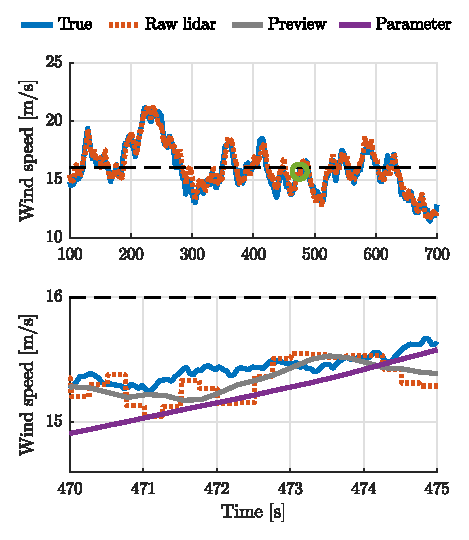
\includegraphics[scale=1.0]{LidarMeas.eps}
	%}
	%                     L B R T
	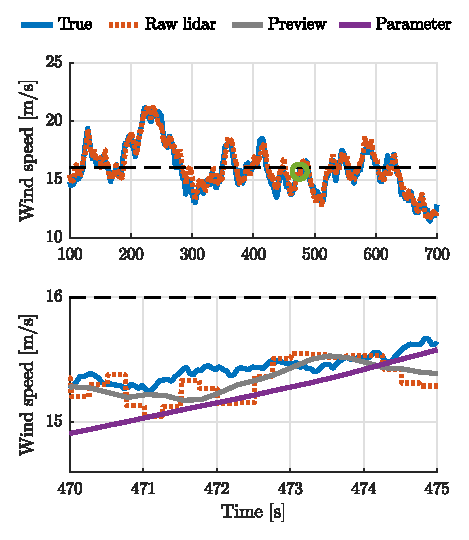
\includegraphics[trim=0 0 0 -5 , clip, scale=1.0]{LidarMeas.eps}
	\caption{Top: true rotor average wind speed and raw rotor average wind speed estimated by lidar. Black dashed line shows mean wind speed. Bottom: close-up of area denoted by green circle in top plot, to show detail. Lower plot includes ideally filtered measurement ($n_\mathrm{filt} = 151$) for preview disturbance and ideally filtered measurement ($n_\mathrm{filt} = 1501$) for preview parameter estimate.}
	\label{fig:lidarmeas}
\end{figure}

\section{CONTROL}\label{sec:Control}
The overarching objective of the wind turbine controller is to minimize the cost of wind energy. Roughly, this translates to maximizing power production while keeping structural loads low. In standard baseline controllers, the generator torque $\tau$ is controlled to maximize power in lower `below rated' winds and the turbine blade pitch angle $\beta$ is used to regulate rotor speed in higher `above rated' winds, thus mitigating excessive structural loading on the wind turbine components \cite{Pao2011CSM}. This study focuses on the latter of these modes (Region III operation). %(see Fig.~\ref{fig:FBD} for a schematic). This study focuses on the latter of these modes (Region III operation). 

\subsection{Linear Parameter-varying Model Predictive Control}\label{subsec:LPVMPC}

In its general form, MPC involves finding a future control trajectory that minimizes a given cost function subject to the plant dynamics and any physical constraints present in the system. MPC is implemented most commonly using a quadratic cost function, linear model, and linear constraints, such that it can be cast as a quadratic program. Our implementation is consistent with this, although we use an LPV model in place of an LTI one for the purpose of designing the LPV MPC. We present only an outline of the LPV MPC law derivation here for brevity, and intend to publish a more comprehensive paper detailing the derivation separately. 
%For brevity, we will not present the entire derivation of the LPV MPC law here: we will instead provide an outline, and intend to publish a more comprehensive paper detailing the derivation separately.

Consider the optimization problem
%\begin{align}
%\underset{x_{k+i},u_{k+i},y_{k+i}}{\text{minimize }} & \sum_{i=0}^{N-1}\left\{ y_{k+i}\tran L y_{k+i} + u_{k+i}\tran R' u_{k+i} \right\} + x_N\tran P x_N \label{eq:DTcost} 
%\end{align}
%\begin{align}
%\text{subject to } & x_{k+i+1} = A_{k+i}x_{k+i} + B_{k+i}u_{k+i} \nonumber\\
%\empty & \hspace{15mm} + B_{dk+i}d_{k+i} - \Delta x^0_{k+i+1, k+i} \label{eq:DTdynamics} \\
%\empty & x_k = x_{k,\mathrm{meas}} \label{eq:InitialCond} \\
%\empty & y_{k+i} = C_{k+i}x_{k+i} + D_{k+i}u_{k+i} \nonumber \\
%\empty & \hspace{15mm} + D_{d{k+i}}d_{k+i} \label{eq:DToutput} \\
%\empty & u_\mathrm{min} \leq u_{k+i} \leq u_\mathrm{max} \label{eq:DTfirstinequality} \\
%\empty & |u_{k+i+1} - u_{k+i}| \leq \Delta u_\mathrm{max} \label{eq:DTlastinequality} \\
%\empty & \hspace{10mm} \forall \: \: i = 0,1,...,N-1. \nonumber 
%\end{align}
\begin{align}
\underset{\tiny{x_{i}, u_{i}, y_{i}}}{\text{minimize }} & \sum_{i=0}^{N-1}\left\{ y_{i}\tran L y_{i} + u_{i}\tran R' u_{i} \right\} + x_N\tran P x_N \label{eq:DTcost} \\
\text{subject to } & x_{i+1} = A_{i}x_{i} + B_{i}u_{i} + B_{di}d_{i} - \Delta x^0_{i+1, i} \label{eq:DTdynamics} \\
\empty & x_0 = x_{k,\mathrm{meas}} \label{eq:InitialCond} \\
\empty & y_{i} = C_{i}x_{i} + D_{i}u_{i} + D_{d{i}}d_{i} \label{eq:DToutput} \\
\empty & u_\mathrm{min} \leq u_i \leq u_\mathrm{max} \label{eq:DTfirstinequality} \\
\empty & |u_{i} - u_{i-1}| \leq \Delta u_\mathrm{max} \label{eq:DTlastinequality} \\
\empty & \hspace{20mm} \forall \: \: i = 0,1,...,N-1. \nonumber 
\end{align}
We use $(A_i,B_i,B_{di},C_i,D_i,D_{di})$ to represent the discrete-time (DT) state-space model of their CT counterparts, evaluated at the parameter value $\gamma_{k+i}$ at the $i$th time step. $\Delta x^0_{i+1, i} \coloneqq x^0_{i+1} - x^0_i$, the difference between the linearization operating points of the models at $\gamma_{k+i+1}$ and $\gamma_{k+i}$. $L \geq 0$, $R' > 0$, and $P > 0$ are weighting matrices, the design of which is discussed shortly. Finally, \eqref{eq:DTfirstinequality} is used in this study to provide a lower saturation limit for blade pitch and an upper saturation limit for generator torque, while \eqref{eq:DTlastinequality} constrains the blade pitch rate.

Condensing the problem \eqref{eq:DTcost}-\eqref{eq:DTlastinequality} by eliminating the states $x_{i}$ from the decision variable leads to the form
\begin{align}
\underset{\mathbf{u}}{\text{minimize}} & \frac{1}{2}\mathbf{u}\tran \mathbf{H}(\Gamma) \mathbf{u} + \mathbf{h}\tran(\Gamma)\mathbf{u} \label{eq:CondensedCost} \\
\text{subject to } &\mathbf{G}(\Gamma)\mathbf{u} \leq \mathbf{g}(\Gamma) \label{eq:CondensedConstraint}
\end{align}
where
\begin{align*}
\mathbf{u} &\coloneqq \begin{bmatrix} u_0\tran & u_{1}\tran & \cdots & u_{N-1}\tran \end{bmatrix}\tran, \hspace{2mm}\text{and} \\
\Gamma &\coloneqq \begin{bmatrix} \gamma_k & \gamma_{k+1} & \cdots & \gamma_{k+N} \end{bmatrix}\tran; 
\end{align*} 
and $\mathbf{H}, \mathbf{h}, \mathbf{G}, \text{ and } \mathbf{g}$ are dependent on various elements of the sparse problem \eqref{eq:DTcost}-\eqref{eq:DTlastinequality}, as listed in Table~\ref{tab:CondensedDependencies}.
%and $\mathbf{H}, \mathbf{h}, \mathbf{G}, \text{ and } \mathbf{g}$ are dependent on various elements of the sparse problem \eqref{eq:DTcost}-\eqref{eq:DTlastinequality}.
\begin{table}[h]
	\caption{Condensed MPC problem dependencies}
	\label{tab:CondensedDependencies}
	\begin{center}
		\begin{tabular}{|c||c|c|c|c|}
			\hline
			 & $\mathbf{H}$ & $\mathbf{h}$ & $\mathbf{G}$ & $\mathbf{g}$\\
			\hline
			Parameter vector $\Gamma$ & \blkdot & \blkdot & \blkdot & \blkdot \\ 
			\hline 
			DT model matrices from \eqref{eq:DTdynamics}-\eqref{eq:DToutput} & \blkdot & \blkdot & \blkdot & \blkdot \\
			\hline
			Cost function matrices $L,R',Q_f$ & \blkdot & \blkdot & \blkdot & \blkdot \\
			\hline
			Current state $x_{k,\mathrm{meas}}$ & \empty & \blkdot & \empty & \blkdot \\
			\hline
			Future disturbances $d_{k+i}$ & \empty & \blkdot & \empty & \blkdot \\
			\hline
			State operating points $x^0_{k+i}$  & \empty & \blkdot & \empty & \blkdot \\
			\hline
			Input operating points $u^0_{k+i}$  & \empty & \empty & \empty & \blkdot \\
			\hline
		\end{tabular}
	\end{center}
\end{table}

Now, let $\mathbf{u} = \mathbf{u'} + \mathbf{c}$, where $\mathbf{u'} = -\mathbf{H}^{-1}(\Gamma)\mathbf{h}(\Gamma)$ is the unconstrained global minimizer of \eqref{eq:CondensedCost}. Problem \eqref{eq:CondensedCost}-\eqref{eq:CondensedConstraint} can then be replaced with 
\begin{align}
\underset{\mathbf{c}}{\text{minimize }} & \frac{1}{2}\mathbf{c}\tran \mathbf{H}(\Gamma) \mathbf{c} \label{eq:CLPCost} \\
\text{subject to } &\mathbf{G}(\Gamma)\mathbf{c} \leq \mathbf{g}(\Gamma) + \mathbf{G}(\Gamma)\mathbf{H}^{-1}(\Gamma)\mathbf{h}(\Gamma), \label{eq:CLPConstraint}
\end{align}
%which is in the so-called `closed-loop paradigm' form: we see that $\mathbf{c} = \mathbf{0}$, the minimizer of \eqref{eq:CLPCost}, is optimal so long as \eqref{eq:CLPConstraint} is satisfied, as expected since this gives $\mathbf{u} = \mathbf{u'}$. Finally, the controls sent to the plant at the $k$th time are simply the first entries of $\mathbf{u} = -\mathbf{H}^{-1}(\Gamma)\mathbf{h}(\Gamma) + \mathbf{c}^\star$ (where $\mathbf{c}^\star$ is the solution to \eqref{eq:CLPCost}-\eqref{eq:CLPConstraint}) offset by the current operating point $u^0_k$.  
which is in the so-called `closed-loop paradigm' form \cite{Rossiter2018}: we see that $\mathbf{c} = \mathbf{0}$, the unconstrained minimizer of \eqref{eq:CLPCost}, is optimal so long as \eqref{eq:CLPConstraint} is satisfied. Finally, the controls sent to the plant at the $k$th time are simply the first entries of $\mathbf{u} = -\mathbf{H}^{-1}(\Gamma)\mathbf{h}(\Gamma) + \mathbf{c}^\star$ (where $\mathbf{c}^\star$ is the solution to \eqref{eq:CLPCost}-\eqref{eq:CLPConstraint}) offset by the current operating point $u^0_k$. 

The running cost matrices $L$ and $R'$ are constructed with $L$, the performance output cost, containing terms penalizing deviations in rotor speed, tower fore-aft motions, and pitching accelerations, and $R'$ penalizing torque and pitch commands \cite{Sinner2018}. The terminal cost matrix $P$ is the positive-definite solution the discrete algebraic Riccati equation \cite{Rawlings2000} for the model evaluated at $\gamma_{k+N}$.
%\begin{align}\label{eq:DARE}
%\begin{split}
% Q_f &= A_{k+N}\tran Q_f A_{k+N} + C_{k+N}\tran L C_{k+N}\\ 
% \empty & \hspace{2mm}-(A_{k+N}\tran Q_f B_{k+N} + C_{k+N}\tran L D_{k+N})(B_{k+N}\tran Q_f B_{k+N} \\
% \empty & \hspace{2mm} +D_{k+N}\tran L D_{k+N} + R')^{-1}(A_{k+N}\tran Q_f B_{k+N} \\
% \empty & \hspace{2mm} +C_{k+N}\tran L D_{k+N})\tran.
% \end{split}
%\end{align}

We note here that $x_{k,\mathrm{meas}}$, the current state of the system used in \eqref{eq:InitialCond}, \eqref{eq:CondensedCost}, \eqref{eq:CondensedConstraint}, and \eqref{eq:CLPConstraint}, is assumed to be measured perfectly (i.e, the MPC algorithm is a state feedback law). In practice, an observer would need to be designed to reconstruct a state estimate $\hat{x}_k$ to replace $x_{k,\mathrm{meas}}$ from measured outputs $\tilde{y}$. %Moreover, the LPV MPC law with disturbance inputs presented here has not been proven to be stable in theory. While our simulations (Sections \ref{sec:SimEnv}-\ref{sec:Results}) have not had any stability issues, this result is empirical and proof of stability is an open research topic.

\subsection{Linear Time-invariant Model Predictive Control}

%The design procedure for LTI MPC can be considered simply as a simplification of that described in Section \ref{subsec:LPVMPC}, where $\gamma$ is constant. However, instead of evaluating the LPV model \eqref{eq:LPV_CT_simple} at the mean wind speed $\gamma = 16$, we use the original 16~m/s DT linear model \eqref{eq:LTI_DT}. All dependencies on the parameter vector $\Gamma$ in Table~\ref{tab:CondensedDependencies} are thus removed, and $\mathbf{H}$, $\mathbf{h}$, $\mathbf{G}$, and $\mathbf{g}$ become time invariant (and can be computed offline). The overall size of the optimization problem \eqref{eq:CLPCost}-\eqref{eq:CLPConstraint} does not change. Notably, $\Delta x^0_{k+i+1,k+i} \equiv 0$ in the LTI case.
The design procedure for LTI MPC is a simplification of that described in Section \ref{subsec:LPVMPC} where $\gamma$ is constant. However, instead of evaluating the LPV model \eqref{eq:LPV_CT_simple} at the mean wind speed $\gamma = 16$, we use the original 16~m/s DT linear model \eqref{eq:LTI_DT}. All dependencies on the parameter vector $\Gamma$ in Table~\ref{tab:CondensedDependencies} are thus removed, and $\mathbf{H}$, $\mathbf{h}$, $\mathbf{G}$, and $\mathbf{g}$ become time invariant (and can be computed offline). The overall size of the optimization problem \eqref{eq:CLPCost}-\eqref{eq:CLPConstraint} does not change. Notably, $\Delta x^0_{k+i+1,k+i} \equiv 0$ in the LTI case.

\subsection{Choice of Prediction Horizon}
Throughout the MPC derivation we have not discussed the selection of the prediction horizon $N$. The terminal cost matrix $P$ technically extends the cost function (and system model) to an infinite horizon \cite{Rawlings2000}, but does so without enforcing constraints \eqref{eq:DTfirstinequality}, \eqref{eq:DTlastinequality}, \eqref{eq:CondensedConstraint}, and \eqref{eq:CLPConstraint} and without taking into account parameter variations and disturbance preview beyond the prediction horizon. Having implemented the controller derived, we proceed to investigate the impact that the choice of $N$ has on controller performance.%the $N$th step or disturbance preview beyond the $N-1$th step. Having implemented the controller derived, we proceed to investigate the impact that the choice of $N$ has on controller performance.

MPC texts for LTI systems \cite{Rossiter2018}\cite{Seborg2011} generally recommend using a horizon length that is long enough to capture significant system dynamics, but not so long as to unnecessarily increase the computational burden of MPC. We have chosen to maintain a fixed controller sampling rate of $f_s = 100$~Hz to be consistent with the baseline controller. This guideline therefore leads us to a horizon length on the order of $N=100$, since significant turbine behaviors tend to happen on the order of seconds (pitch actuator, tower fore-aft, blade flap, and rotor motions). Although we might reasonably expect this guideline to extend to the LPV system, the impact of advance preview information is not clear. As such, we test various horizons ranging from $N = 1$ (0.01~seconds of preview) to $N = 200$ (2~seconds of preview). We consider ourselves to be constrained on the upper end by the focus distance of the lidar, which provides a maximum of around 5~seconds of preview information for Region III winds ($N_\mathrm{max} = 500$), but found that prediction horizons $N > 200$ led to unreasonable computation times. 

We note that theoretical works on linear MPC provide methods for choosing prediction horizons that ensure stability and recursive feasibility of the nominal case \cite{Rossiter2018}\cite{Rawlings2000}. Here, we are considering an applied study for preview-enabled input-constrained LPV MPC where the model does not match the plant perfectly, but in doing so, forgo the proven assurance of stability.

\subsection{Processing Preview Measurements}

Since the focus distance of the lidar is fixed, increasing $N$ decreases the time available for processing the noisy lidar measurements. We use a simple moving average filter but advance the output by the (frequency independent) group delay to avoid problems with delayed measurements. The resulting noncausal filter has the transfer function
\begin{equation}\label{eq:mafilter_nc}
H(z) = \frac{1}{n_\mathrm{filt}}\frac{z^{n_\mathrm{filt}-1} + z^{n_\mathrm{filt}-2} + \cdots + z + 1}{z^{\left(n_\mathrm{filt}-1\right)/2}} 
\end{equation}
where $n_\mathrm{filt}$ is the number of samples in the moving average, and must be an odd positive integer. This procedure requires that there is enough time between when the measurement is made by the lidar and when it enters the prediction horizon to advance the averaged measurement appropriately (Fig.~\ref{fig:horizons}).

Simley \& Pao \cite{SimleyPao2015} suggest that longitudinal coherence between the wind field as measured by the lidar and the wind field encountered by the turbine is low for turbulent structures above 0.3~Hz at the focus distance we are considering (approximately 100~m). Using a sample time of 0.01~seconds, the noncausal moving averge filter with $n_\mathrm{filt} = 151$ rolls off at about 0.3~Hz. Therefore, for different values of $N$, we choose $n_\mathrm{filt}$ according to $n_\mathrm{filt} = \mathrm{min}\{151, 2(N_\mathrm{max} - N)+1\}$.

We similarly need to filter the lidar measurement to provide the scheduling parameter $\gamma$. To keep the {\color{black}scheduling parameter `smooth', we say (somewhat arbitrarily) that the desired roll-off in frequency content in $\gamma$ is 0.03~Hz}, a decade below the roll-off of the preview filter. This corresponds to a noncausal moving average filter \eqref{eq:mafilter_nc} with $n_\mathrm{filt} \approx 1501$. Since $(1501-1)/2 \geq N_\mathrm{max} = 500$, we choose $n_\mathrm{filt} = 2(N_\mathrm{max} - N)+1$ in all prediction horizon length test cases. An example of the `ideally' filtered measurements ($n_\mathrm{filt} = 151$ for preview disturbance estimates and $n_\mathrm{filt} = 1501$ for preview parameter estimates) is shown in Fig.~\ref{fig:lidarmeas} (bottom). 

\subsection{Baseline Controller}

A controller provided by our sponsor is used as a reference. The controller is representative of an industry-standard feedback-based law, which predominantly uses generator torque control in below-rated conditions and collective pitch (CP) control above rated. 


\section{SIMULATION ENVIRONMENT}\label{sec:SimEnv}

The focus of this study is on Region III behavior. As such, we test the controllers on a set of six turbulent wind fields (turbulence intensity 15\%) with a mean wind speed of 16~m/s (well into Region III for the turbine in question) and vertical shear with a power law exponent of 0.3. The wind fields were generated using a Kaimal turbulence model defined by Normal Turbulence Model Class B \cite{Jonkman2009}. Each simulation represents 700~seconds of operation for the turbine. To minimize the impact of unrealistic transient behaviors on our results, we remove the first 100~seconds of data, leaving us with a 10-minute record for each wind field.

\section{RESULTS}\label{sec:Results}

\subsection{LTI vs. LPV MPC}
The main difference between the control laws used in our previous study \cite{Sinner2018} and the present work is in the nature of the model. This study uses an LPV model in comparison to the LTI model of the previous work. Figs.~\ref{fig:GS_ltivs}-\ref{fig:B1_ltivs} show some of the differences in performance using the LPV as opposed to the LTI model. Fig.~\ref{fig:GS_ltivs} presents the generator speed regulation performance in terms of error percentage, while Fig.~\ref{fig:B1_ltivs} shows the normalized relative blade pitch angle $\left(\beta - \beta_\mathrm{nom}\right)/ \beta_\mathrm{nom}$, where $\beta_\mathrm{nom}$ is the nominal blade pitch angle for steady 16~m/s winds. Again, absolute values are left out for information privacy reasons.
\begin{figure}[thbp]
	\centering
	\mbox{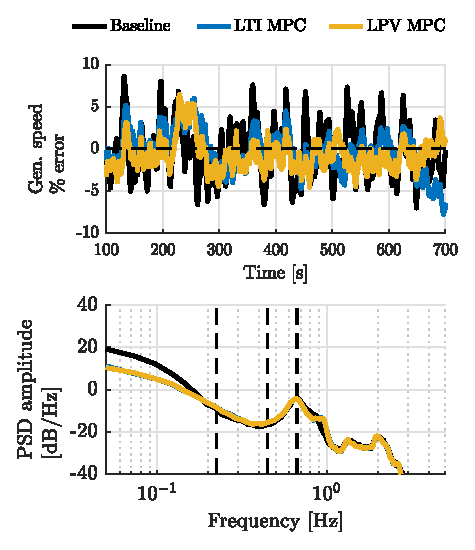
\includegraphics[scale=1.0]{GS_ltivs.eps}
	}
	\caption{Generator speed regulation error of various controllers: baseline control, LTI MPC, and LPV MPC. Upper plot shows time series results for a single wind field, with the rated generator speed shown in black dash. Lower plot displays the power spectral density (PSD) averaged across six wind fields, with black dashed lines at the once-per-rotor revolution (1P), 2P, and 3P frequencies (from left to right).}
	\label{fig:GS_ltivs}
\end{figure}
\begin{figure}[thbp]
	\centering
	\mbox{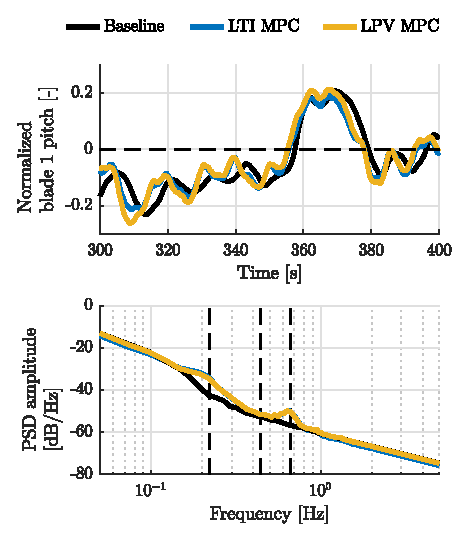
\includegraphics[scale=1.0]{B1_ltivs.eps}
	}
	\caption{Normalized relative blade pitch angle for various controllers: baseline control, LTI MPC, and LPV MPC. Upper plot shows a subset of the time series results for a single wind field, with the nominal 16~m/s blade pitch angle shown in black dash. Lower plot is the PSD averaged across six wind fields, with black dashed lines at the 1P, 2P, and 3P frequencies (from left to right).}
	\label{fig:B1_ltivs}
\end{figure}

We see that, using the same cost functions and operating at mean wind speeds that align with the linearization point of the LTI model, the LTI and LPV MPCs behave comparably. However, from Figs.~\ref{fig:lidarmeas} (top) and \ref{fig:GS_ltivs} (top), we see that the LTI MPC's performance worsens significantly at times when the rotor average wind speed deviates significantly from the linearization point of the LTI model, as happens at 650-700~seconds. 

\subsection{Prediction Horizon Length Testing}
In varying the prediction horizon for MPC, we limit both the controller's awareness of physical constraints and its knowledge of disturbances and, in the LPV case, parameter variations outside of the finite horizon. A major trade off in the MPC formulation is between prediction horizon length and computational burden of the nonlinear control law. Textbooks \cite{Rossiter2018}\cite{Seborg2011} suggest choosing a horizon that is just long enough to provide good performance (particularly compared to long horizon cases) when there is no information about future disturbances. This is clearly a heuristic, and may differ significantly for different systems. By testing various prediction horizon lengths $N \in \{1, 2, 5, 10, 20, 50, 100, 200\}$, corresponding to 0.01, 0.02, 0.05, 0.1, 0.2, 0.5, 1, and 2~seconds of prediction, we hope to provide some insight to the trade-off between prediction horizon length and computational burden for preview-enabled wind turbine MPC.    

We have not made significant efforts in this work to solve the dense quadratic program \eqref{eq:CLPCost}-\eqref{eq:CLPConstraint} efficiently. As such, we will use as an indicator of the complexity the problem size, rather than computation time. For both LTI and LPV MPC, the size of the optimization variable is $\mathrm{dim}\:(\mathbf{c}) = mN = 2N$ and the number of constraints is $\mathrm{dim}\:(\mathbf{g}) = 4N$. We note that the case $N = N_\mathrm{max} = 500$ was not tested thoroughly because the computation time was too great. As measures of the performance of the controllers, we use generator speed root mean square error (RMSE); tower base fore-aft moment damage equivalent load (DEL) \cite{Hayman2012}; and RMS pitch actuator velocity as percentages of the baseline controller value. These quantities are averaged across the six wind fields to give the final statistic, which is shown in Fig.~\ref{fig:bargraph}. 

The results obtained are a far cry from the expected poorer performance of lower horizon length MPCs. While this trend is, arguably, present for the LTI MPC case, there is no clear evidence that longer horizons lead to better performance for the LPV MPC: although generator speed regulation does show very slight improvements with increasing horizon length, this comes at the cost of increased pitch actuator usage. Tower base fore-aft moment DEL is lowest for $N = 50$, but results for $1 \leq N < 50$ are not significantly worse.

\begin{figure}[thbp]
	\centering
	\mbox{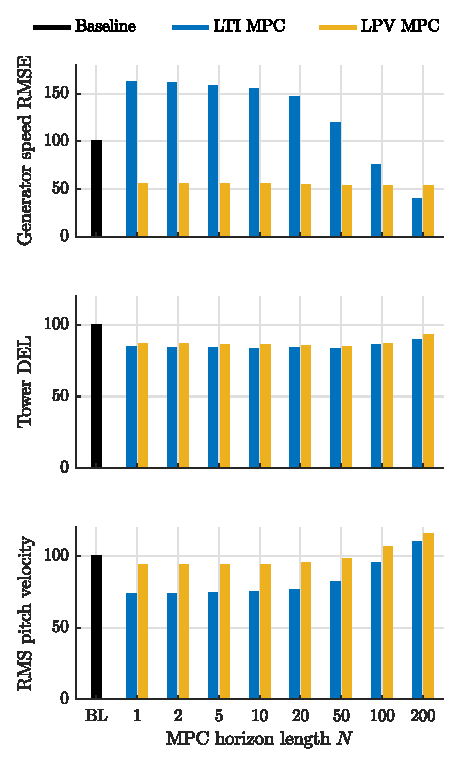
\includegraphics[trim=0 0 0 -5, clip, scale=1.0]{effectofN.eps}
	}
	\caption{Cost metrics for the LTI and LPV MPCs for various prediction horizon lengths as percentages of the baseline controller (BL) performance.}
	\label{fig:bargraph}
\end{figure}

There are several possible explanations for this surprising behavior. A contributing factor may be the level to which the lidar data is filtered, particularly for the scheduling parameter. Larger $N$ means that the filter whose output $\gamma$ is used to schedule the model has a higher bandwidth, which can lead to more erratic changes in the MPC operating point and higher than necessary pitch motions. However, one could consider the LTI MPC as an extreme case of low-pass filtering the parameter estimate (so that only the DC component remains), and as is evident in generator speed regulation performance in particular, behavior of the LTI MPC is worse than LPV MPC for short horizons. Part of this deterioration could be from the implicit assumption in forming $P$ that $d_{i} = 0\:\forall\:i>N-1$: for LPV MPC, this assumption is reasonable since both the scheduling parameter and disturbance preview $d_k$ are filtered versions of the same signal; however, for LTI MPC, the change from $d_{N-1}$ to zero at the final prediction time could be large. This suggests that there may be an `ideal' order for the moving average filter $H(z)$ that lies somewhere in the interval $999 < n_\mathrm{filt} < \infty$ (where $n_\mathrm{filt} = 999$ is the maximum filter order possible given the lidar focus distance), but this sweet spot is not investigated in this research. If such an ideal $n_\mathrm{filt}$ exists, it could be used to inform a good focus distance for the lidar.

We also point out that the MPC is implemented over a nonlinear plant (which differs significantly from the LTI or LPV models used by the controller). The MPC algorithm propagates the model forward over the prediction horizon in open loop, and large discrepancies between the prediction and actual nonlinear plant behavior can occur, particularly for longer horizons. The effect of large prediction errors can mean that control inputs $u_{k+i}, i \gg 1$ are not useful. Moreover, large discrepancies could cause an optimal solution that exchanges good (but erroneous) performance in the long horizon for poorer performance in the short horizon. It seems plausible that the increase in pitching behavior for longer horizons could be a result of this sort of effect.

It is also important to note that the cost function matrices $L$ and $R'$ were kept constant for this study. All results presented here rely heavily on the cost function chosen, and different weightings will lead to different trade-offs in behavior. For instance, the very poor generator speed regulation seen for short horizon LTI MPC could probably be improved by choosing different weights, but this will likely come at the cost of tower loading and blade pitch performance.

Although the results we present here are surprising, they are very promising for real-time MPC implementation. LPV MPC outperforms the baseline control in all cost metrics for $N < 100$, and we see little to no deterioration in this performance as horizons becomes very short. This means that we may be able to choose very short (and computationally efficient) horizons for LPV MPC, and running such a controller in real time is entirely possible.

\section{CONCLUSIONS AND FUTURE WORK}\label{sec:Concl}

The results of this paper perhaps pose more questions than they answer. In particular, we are yet to provide a conclusive answer as to why shorter horizons tend to improve, or at least not cause deterioration of, LPV MPC performance. We have proposed some possible answers, but further research is needed to confirm these hypotheses. In any case, it is clear that LPV MPC, even with short horizons, can reduce generator speed regulation errors and tower loading as compared to a baseline controller while also decreasing pitch activity.

Our research intent is to continue to investigate various aspects of the MPC formulation and their impacts on the performance of wind turbine MPC. The next major focus is on developing MPC for below-rated and transition wind speeds, so that the LPV MPC can cover the entire operational envelope of a wind turbine.
   

%\addtolength{\textheight}{-0cm} %{-12cm}  % This command serves to balance the column lengths
                                  % on the last page of the document manually. It shortens
                                  % the textheight of the last page by a suitable amount.
                                  % This command does not take effect until the next page
                                  % so it should come on the page before the last. Make
                                  % sure that you do not shorten the textheight too much.

%%%%%%%%%%%%%%%%%%%%%%%%%%%%%%%%%%%%%%%%%%%%%%%%%%%%%%%%%%%%%%%%%%%%%%%%%%%%%%%%
\bibliography{ACC19refs}
\bibliographystyle{IEEEtran}

\end{document}
